\chapter{System response}
\section{Dynamics}
\label{a:dynamics_response}
Following are figures detailing the complete system response of the full car dynamic model to two different situations. The first situation (figure \ref{fig:2cm_straight}) is the vehicle driving directly into a raised 2cm bump. As can be seen there is no roll created in this system. In the second situation (figure \ref{fig:2cm_ramp}) the vehicle drives over the side of the same obstacle so one side remains on the ground and the other drives directly up the 2cm bump. In this system, the roll can be clearly seen.

\begin{figure}[t]
	\centering
	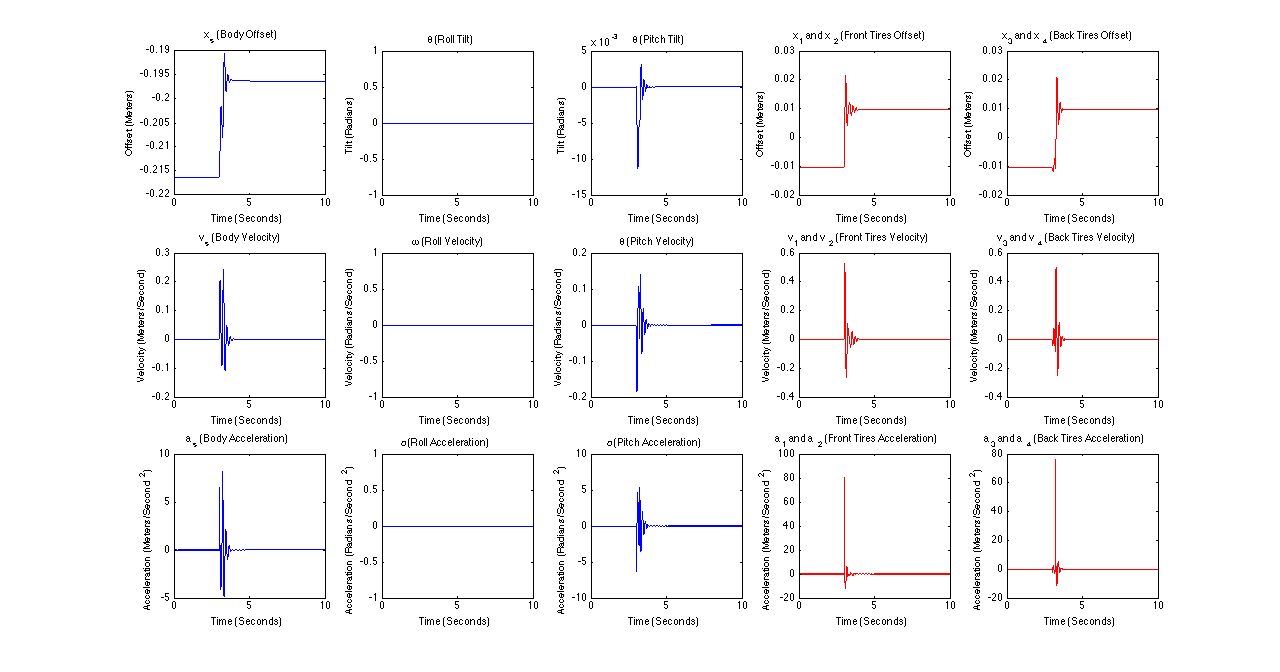
\includegraphics[width=1\textwidth]{figures/fullcar_2cm_straight.png}
	\caption{The dynamics response of a full car driving directly into a 2cm bump.}
	\label{fig:2cm_straight}
\end{figure}

\begin{figure}[t]
	\centering
	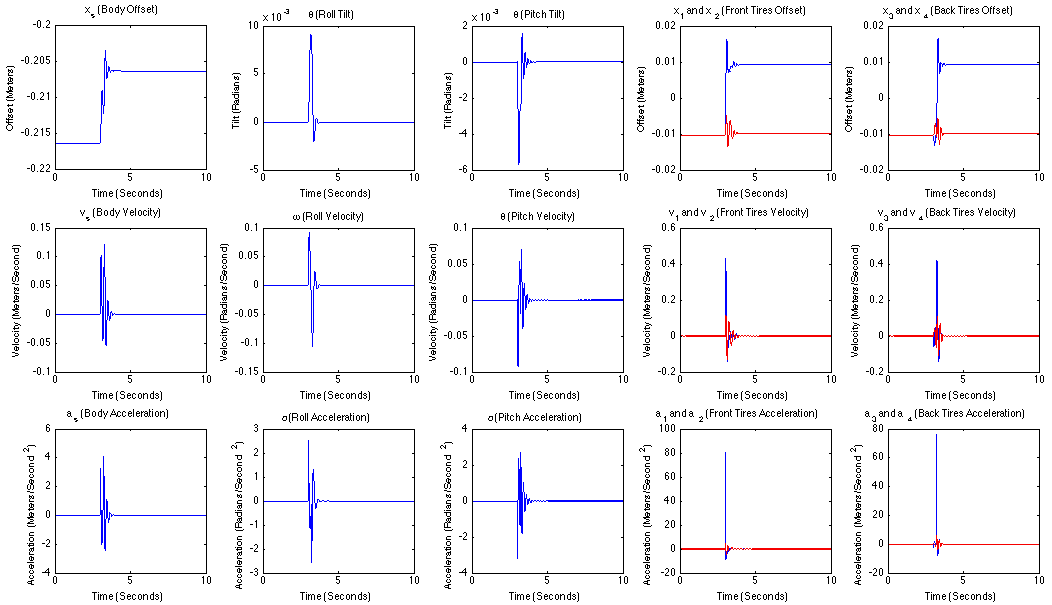
\includegraphics[width=1\textwidth]{figures/fullcar_2cm_ramp.png}
	\caption{The dynamics response of a full car driving into the side of a 2cm bump.}
	\label{fig:2cm_ramp}
\end{figure}

\section{Inverse dynamics}
Following are the figures detailing the complete system response of a full car as viewed by a following vehicle. The lead vehicle executes the same two maneuvers as in appendix \ref{a:dynamics_response}, and the trailing car follows and records. As in figure \ref{fig:2cm_straight}, figure \ref{fig:2cm_straight_inv} exhibits no roll as the vehicle drives directly over the bump. However, figure \ref{fig:2cm_ramp_inv} clearly shows the roll that the leading car is experiencing as it drives over the edge of the 2cm bump.

\begin{figure}[t]
	\centering
	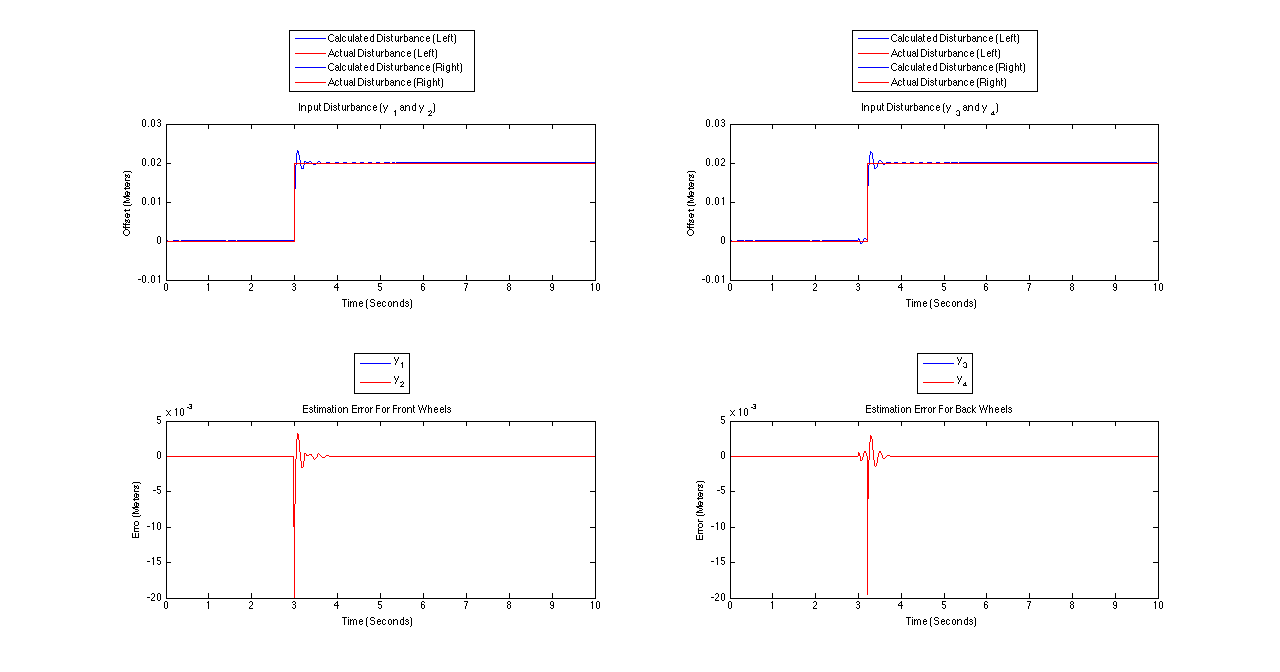
\includegraphics[width=1\textwidth]{figures/fullcar_2cm_straight_inverse.png}
	\caption{The inverse dynamics response of a full car driving directly into a 2cm bump.}
	\label{fig:2cm_straight_inv}
\end{figure}

\begin{figure}[t]
	\centering
	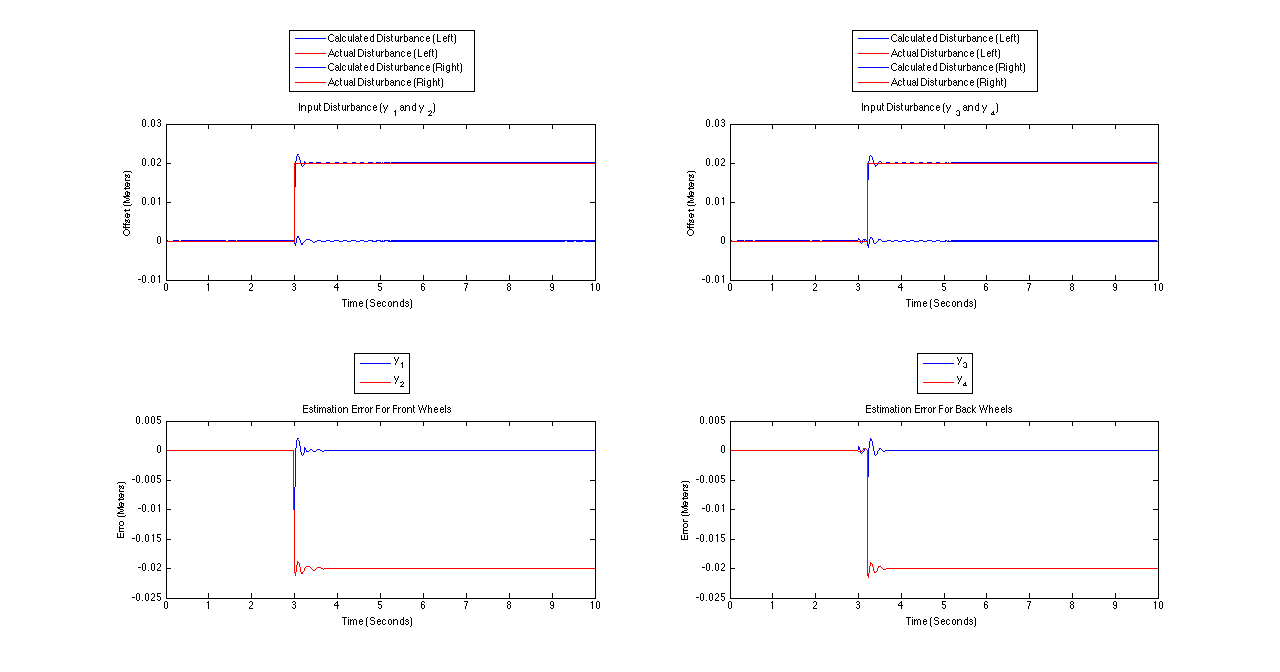
\includegraphics[width=1\textwidth]{figures/fullcar_2cm_ramp_inverse.png}
	\caption{The inverse dynamics response of a full car driving into the side of a 2cm bump.}
	\label{fig:2cm_ramp_inv}
\end{figure}

